\section{ZFC 公理集合论}

为了消解罗素悖论,需要限制概括公理模式。为此,数理学家 Zermelo 和 Fraenkel 提出了一套公理定义集合,称为 \textbf{ZF 公理集合论(ZF Axiomatic Set Theory)},在 ZF 公理集合论的基础上加上\textbf{选择公理(Axiom of Choice)}就是 \textbf{ZFC 公理集合论}。ZFC 公理集合论一共有九条公理:

\begin{enumerate}
    \item \textbf{外延公理 Axiom of extensionality}:设 $A,B$ 是集合,说 $A$ 和 $B$ 是相等的,记作 $A = B$,当且仅当,两个集合有相同的元素。
    \item \textbf{配对公理 Axiom of pairing}:对于任意集合(或元素) $a,b$,存在一个集合 $\{a,b\}$ 包含 $a,b$。
    \item \textbf{分类公理模式 Axiom schema of specification}:设 $ A $ 是一个集合,并对于每个 $ x\in A $,设 $ P(x) $ 是一个关于 $ x $ 的性质。那么存在一个集合 $ \{x\in A:P(x)\} $,它的元素是 $ A $ 中使 $ P(x) $ 成立的所有 $x$。
    \item \textbf{并集公理 Axiom of union}:对于集合 $ A $,存在集合 $ \cup A $。$ \forall u \in \cup A $,存在集合 $ B\in A $,使得 $ u\in B $。
    \item \textbf{幂集公理 Axiom of power set}:对于集合 $ A $,存在集合 $ \mathcal{P}(A) $ 是所有 $ A $ 的子集的集合,称为幂集。
    \item \textbf{无穷公理 Axiom of infinity}:存在集合 $ A $,使得$ \varnothing \in A $,且任意对象 $ a\in A $ 都有 $ a\cup \{a\}\in A $。
    \item \textbf{替代公理模式 Axiom schema of replacement}:设属性 $ P(x,y) $,对于每个 $ x $ 唯一确定一个 $ y $ 使得 $ P(x,y) $ 成立。则对于任意集合 $ A $,存在集合 $ B $,任意 $  b\in B $,存在 $ a\in A $ 使得 $ P(a,b) $ 成立。
    \item \textbf{正则公理 Axiom of regularity}:任意非空集合 $ A $ 包含一个元素 $ x  $,使得 $ x\cap A = \varnothing $。
    \item \textbf{选择公理 Axiom of choic}:任意由非空集合组成的集族 $ \mathcal{F} $,存在一个选择函数 $ f $,使得对每个 $ A\in\mathcal{F} $,有 $ f(A)\in A $。
\end{enumerate}

\subsection{外延公理}

\begin{axiom}[外延公理 Axiom of extensionality]
    设 $A,B$ 是集合,说 $A$ 和 $B$ 是相等的,记作 $A = B$,当且仅当,两个集合有相同的元素。
\end{axiom}

\begin{note}
    外延公理说明一个集合完全由它的元素决定。通过外延公理,可以定义子集。
\end{note}
\vspace{1em}

\subsubsection{子集}
\begin{definition}[子集 Subset]
    设 $ A,B $ 是集合,说 $ A $ 是 $ B $ 的子集,记作 $ A\subseteq B $,当且仅当,$ A $ 的每个元素都是 $ B $ 中的元素。
\end{definition}

\begin{theorem}
    若两个集合互为对方的子集,两集合相等。也即,设 $ A,B $ 是集合,如果 $ A\subseteq B $ 且 $ B\subseteq A $,则 $ A = B $。
\end{theorem}

\subsection{配对公理}

\begin{axiom}[配对公理 Axiom of pairing]
    对于任意集合(或元素) $a,b$,存在一个集合 $\{a,b\}$ 包含 $a,b$。
\end{axiom}

\begin{note}
    外延公理和配对公理说明,集合中的元素都是独一无二的,且没有顺序,比如:
    \[  
        \{1,2\} = \{2,1\} ,\  \{1,1\} = \{1\} 
    \]
    通过配对公理,可以定义有序对。
\end{note}

\subsubsection{有序对}
\begin{definition}[有序对 Ordered Pair]
    由两个元素 $ x $ 和 $ y $ 按一定顺序排列成的二元组称为一个有序对或序偶,记为:$ (x,y) $,其中 $ x $ 是它的第一个元素,$ y $ 是第二个,那么
    \[
        (x,y) := \{x,\{x,y\}\}
    \]
\end{definition}
\vspace{1em}

\begin{proposition}[有序对的性质]
    设 $x,y$ 是元素,$(x,y)$ 是有序对,那么
    \begin{enumerate}
        \item 当 $ x= y $ 时,$ (x,y)=(y,x) $;当 $ x\neq y $ 时,$ (x,y)\neq(y,x) $
        \item $ (x,y)=(u,v) $ 当且仅当 $ x=u,\ y=v $
    \end{enumerate}
\end{proposition}
\vspace{1em}

\begin{definition}[有序数组 Ordered n-Tuple]
    由 $ n $ 个元素 $ x_1,x_2,\cdots,x_n $ 按一定顺序排列成的 $ n $ 元组称为一个有序数组,记为:$ (x_1,x_2,\cdots,x_n) $,其中 $ x_1 $ 是它的第一个元素,$ x_2 $ 是第二个,依此类推,那么
    \[
        (x_1,x_2,\cdots,x_n) := ((x_1,x_2,\cdots,x_{n-1}),x_n)
    \]
\end{definition}
\vspace{1em}

\begin{proposition}
    两个 $ n $ 元有序数组 $ (a_1,\cdots,a_n)=(b_1,\cdots,b_n) $ 相等,当且仅当,$ a_1=a_1,\cdots,a_n=b_n $
\end{proposition}

\subsection{分类公理模式}

\begin{axiom}[分类公理模式 Axiom schema of specification]
    设 $ A $ 是一个集合,并对于每个 $ x\in A $,设 $ P(x) $ 是一个关于 $ x $ 的性质。那么存在一个集合 $ \{x\in A:P(x)\} $,它的元素是 $ A $ 中使 $ P(x) $ 成立的所有 $x$。
\end{axiom}

\begin{note}
    分类公理模式是 ZFC 公理集合论中构造集合的方式,与朴素集合论的概括公理模式相比,它是从一个已知集合中挑选元素构造一个子集,而不是直接构造所有满足性质 $ P $ 的集合。因此通过分类公理模式可以定义空集、交集、差集、补集…… 但不能定义并集。并集需要从已知集合构造一个更大的,包含已知集合的集合,这需要并集公理。
\end{note}

\subsubsection{空集}

\begin{definition}[空集 Empty ]
    对于任意集合 $ A $,集合:
    \[
        \{x\in A:x\neq x\} 
    \]
    称为空集,记为 $ \varnothing $
\end{definition}

\begin{note}
因为满足性质 $ x\neq x $ 的元素并不存在,所以 $ \varnothing $ 中不包含任何元素。根据定义,空集是任意集合的子集。
\end{note}

\subsubsection{交集}
\begin{definition}[交集 Intersection]
    两个集合 $ A $ 和 $ B $ 的交是一个集合,记为 $ A\cap  B $,那么
    \[
        A\cap B := \{x\in A : x\in B\} 
    \]
\end{definition}

\begin{figure}[htbp]
    \centering
    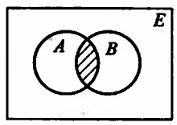
\includegraphics[width=0.2\textwidth]{figures/chapter1/chapter1_1} 
    \caption{交集}
    \label{fig:chapter1_1}
\end{figure}

\begin{definition}[分离 Disjoint]
    两个集合 $ A $ 和 $ B $ 是分离的,当且仅当:$ A\cap B = \varnothing $
\end{definition}

\subsubsection{差集}

\begin{definition}[差集 Difference]
    两个集合 $ A $ 和 $ B $ 的差是一个集合,记为 $ A-  B $,那么
    \[
        A-  B := \{x\in A:x\notin B\}
    \]
\end{definition}

\begin{figure}[htbp]
    \centering
    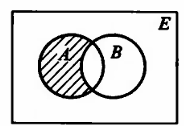
\includegraphics[width=0.2\textwidth]{figures/chapter1/chapter1_2} 
    \caption{差集}
    \label{fig:chapter1_2}
\end{figure}

\newpage
\subsubsection{补集}
\begin{definition}[补集]
    设集合 $ E $ 和 $ A $,$ A\subseteq E $,$ A $ 的补集记为 $ \complement_EA $,那么
    \[
        \complement_EA := E - A = \{x\in E:x\notin A\}
    \]
\end{definition}

\begin{figure}[htbp]
    \centering
    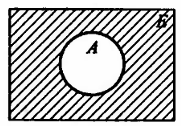
\includegraphics[width=0.2\textwidth]{figures/chapter1/chapter1_3} 
    \caption{补集}
    \label{fig:chapter1_3}
\end{figure}

\subsection{并集公理}
\begin{definition}[并集 Union]
    两个集合 $ A $ 和 $ B $ 的并是一个集合,记为 $ A \cup B $,那么
    \[
        A\cup B := \{x:x\in A\ or\ x\in B\} 
    \]
\end{definition}

\begin{figure}[htbp]
    \centering
    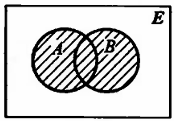
\includegraphics[width=0.2\textwidth]{figures/chapter1/chapter1_4} 
    \caption{并集}
    \label{fig:chapter1_4}
\end{figure}

\begin{definition}[对称差 Symmetric Difference]
    两个集合 $ A $ 和 $ B $ 的对称差是一个集合,记为 $ A \oplus  B $,那么:
    \[
        A\oplus  B := (A-B) \cup (B-A) 
    \]
\end{definition}

\begin{figure}[htbp]
    \centering
    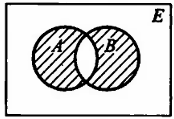
\includegraphics[width=0.2\textwidth]{figures/chapter1/chapter1_5} 
    \caption{并集}
    \label{fig:chapter1_5}
\end{figure}

\begin{theorem}[集合常用算律]
    设 $A,B,C$ 是集合
    \begin{enumerate}
        \item 幂等律: $A\cup A = A,\  A\cap A = A$
        \item 结合律:$A\cup (B\cup C) = (A\cup B)\cup C,\ A\cap(B\cap C) = (A\cap B)\cap C$
        \item 交换律:$A\cup B = B\cup A,\ A\cap B = B\cap A$
        \item 分配律:$ A\cup (B\cap C) = (A\cup B)\cap(A\cup C),\ A\cap (B\cup C) = (A\cap B)\cup(A\cap C) $
        \item 排中律:$A\cup \complement_EA = E$
        \item 矛盾律:$A\cap \complement_EA = \varnothing$
        \item 德摩根律:
        \begin{enumerate}
            \item $A-(B\cup C) = (A-B)\cap (A-C)$
            \item $A-(B\cap C) = (A-B)\cup (A-C)$
            \item $\complement_E(B\cup C) = \complement_EB\cap \complement_EC$
            \item $\complement_E(B\cap C) = \complement_EB\cup \complement_EC$
        \end{enumerate}
        \item 双重否定率:$ \complement_E(\complement_E A) = A $
    \end{enumerate}
\end{theorem}

\subsection{幂集公理}

\begin{axiom}[幂集公理 Axiom of power set]
    对于集合 $ A $,存在集合 $ \mathcal{P}(A) $ 是所有 $ A $ 的子集的集合,称为幂集。
\end{axiom}

\begin{note}
    换句话说,集合 $ A $ 的幂集是 $ A $ 全体子集构成的集合。通过幂集公理,同样可以从已知集合构造更大的集合。 有序对的定义:
    \[
        (a,b) := \{a,\{a,b\}\} 
    \]

    如果 $ a\in A,b\in B $,那么:
    \[
        (a,b)\in \mathcal{P}(\mathcal{P}(A\cup B))
    \]
    通过并集公理和幂集公理,构造集合 $ \mathcal{P}(\mathcal{P}(A\cup B)) $,通过分离公理模式,分离出有序对的集合,从而可以定义两个集合的\textbf{笛卡尔积}。
\end{note}

\subsubsection*{笛卡尔积}

\begin{definition}[笛卡尔积 Cartesian Product]
    设 $ A,\ B $ 为集合,$ A,B $ 的笛卡尔积记为 $ A\times B $,那么
    \[
        A\times B := \{(x,y)\in \mathcal{P}(\mathcal{P}(A\cup B)):x\in A,y\in B\} 
    \]
    递归地,可以定义 $n$ 个集合 $S_1,S_2,\cdots,S_n$ 的笛卡尔积,记为 $\prod^n_{i=1}S_i$,那么
    \[
        (x_1,x_2,\cdots,x_n) \in \prod^n_{i=1}S_i
    \]
\end{definition}


\begin{figure}[htbp]
    \centering
    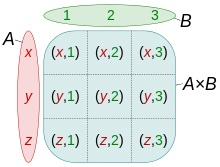
\includegraphics[width=0.2\textwidth]{figures/chapter1/chapter1_6} 
    \caption{笛卡尔积}
    \label{fig:chapter1_6}
\end{figure}

\begin{note}
    笛卡尔积是构造有序对集合的基本方法。有了有序对的集合,再通过分离公理模式,从中分离出我们感兴趣的有序对,从而构建起集合元素之间的关系,从而为集合定义各种结构。
\end{note}

\begin{proposition}[笛卡尔积的性质]
    设 $A, B, C$ 为集合,
    \begin{enumerate}
        \item 笛卡尔积不满足结合律
        \begin{enumerate}
            \item $(A\times B)\times C \neq A\times (B\times C)$
        \end{enumerate}
        \item 笛卡尔积通常不满足交换律
        \begin{enumerate}
            \item $A\times B \neq B\times A$
        \end{enumerate}
        \item 笛卡尔积对集合交并满足分配律
        \begin{enumerate}
            \item $A \times(B \cup C)=(A \times B) \cup(A \times C)$
            \item $(B \cup C) \times A=(B \times A) \cup(C \times A)$
            \item $A \times(B \cap C)=(A \times B) \cap(A \times C) $
            \item $(B \cap C) \times A=(B \times A) \cap(C \times A)$
        \end{enumerate}
    \end{enumerate}
\end{proposition}

\subsection{无穷公理}

\begin{axiom}[无穷公理 Axiom of Infinity]
    存在集合 $ A $,使得 $ \varnothing \in A $,且任意对象 $ a\in A $ 都有 $ a\cup \{a\}\in A $
\end{axiom}

\begin{note}
    无穷公理断言了无穷集的存在,但这种“无穷”并不是像朴素集合论那样不加限制的无穷,而是对后继(successor)操作 $ a\cup \{a\} $ 封闭的无穷,也即 $ \forall a \in A $ 都存在其后继 $ a\cup \{a\}\in A $。满足这一性质的集合,也称为\textbf{归纳集(Inductive Set)}。自然数的递归定义依赖于无穷公理。数学归纳法的有效性依赖于自然数集的无限性。若没有无穷公理,归纳法只能应用于有限步骤。
\end{note}

\subsubsection*{自然数}

\begin{definition}[自然数 Natural numbers]通过无穷公理,我们可以无限递归地定义每一个自然数:
    \begin{enumerate}
        \item 令 $ 0:=\varnothing $
        \item 任意自然数 $n$ 的后继 $ S(n) $,那么 $ S(n) := n\cup \{n\} $
    \end{enumerate}
    无穷公理说明,集合 $ n\cup \{n\} $ 的存在,记所有自然数的集合记为 $ \mathbb{N} $。
\end{definition}

\begin{definition}[自然数的序]
    设 $ \forall m,n\in\mathbb{N} $ 是自然数,我们说 $ n $ 大于等于 $ m $,记作 $ n\ge m $ 或 $ m\le n $,当且仅当 $ m\subseteq n $。
\end{definition}

\begin{example}
    根据自然数的定义,
    \begin{align*}
        0 &= \{\} = \varnothing\\
        1 &= 0\cup \{0\} = \{0\} = \{\varnothing\}\\
        2 &= 1\cup \{1\} = \{0,1\} = \{\varnothing,\{\varnothing\}\}\\
        3 &= 2\cup \{2\} = \{0,1,2\} = \{\varnothing,\{\varnothing\},\{\varnothing,\{\varnothing\}\}\}\\
        \vdots
    \end{align*}
\end{example}

\vspace{1em}

\subsection{替代公理模式}

\begin{axiom}[替代公理模式 Axiom Schema of Replacement]
    设属性 $ P(x,y) $,对于每个 $ x $ 唯一确定一个 $ y $ 使得 $ P(x,y) $ 成立。则对于任意集合 $ A $,存在集合 $ B $,任意 $  b\in B $,存在 $ a\in A $ 使得 $ P(a,b) $ 成立。
\end{axiom}

\begin{note}
    属性 $ P(x,y) $ 类似于“函数”(因为函数是通过集合公理定义的,所以在集合公理中避免谈及“函数”),也即 $ x $ 对应唯一的 $ y $。通过替代公理模式,可以将已知集合 $ A $ 中的元素 $ x $ 替换为 $ y $ 生成一个新的集合 $ B $。通过替代公理模式,可以递归地定义自然数的加法与乘法。
\end{note}

\vspace{1em}

\subsubsection*{自然数的加法与乘法}

\begin{definition}[自然数的加法]
    设 $m$ 是自然数,
    \begin{enumerate}
        \item $ m+0:=m $
        \item 任意自然数 $ n $ 的后继为 $ S(n) $,$ m+S(n):=S(m+n) $
    \end{enumerate}
\end{definition}

\begin{note}
    替代公理模式断言了属性,$P(m,0)=m+0$ 和 $P(m,n)=m+S(n)$ 的存在,再根据无穷公理,可以递归的定义任意自然数 $m$ 与 $n$ 的加法:
    \begin{align*}
        m+0 &= m\\
        m+1 &= m+S(0) = S(m+0)= S(m)\\
        m+2 &= m+S(1) = S(m+1)=S(S(m+0))=S(S(m))\\
        m+3 &= m+S(2) = S(m+2)=S(S(S(m+0)))=S(S(S(m)))\\
        \vdots
    \end{align*}
\end{note}
\newpage

\begin{definition}[自然数的乘法]
    设 $m$ 是自然数,
    \begin{enumerate}
        \item $ m\times 0:=0 $
        \item 任意自然数 $ n $ 的后继为 $ S(n) $, $m\times S(n):=m\times n+m$
    \end{enumerate}
\end{definition}

\begin{note}
     替代公理模式断言了属性,$P(m,0)=m\times 0$ 和 $P(m,n)=m\times S(n)$ 的存在,再根据无穷公理,可以递归的定义任意自然数 $m$ 与 $n$ 的乘法:
     \begin{align*}
        m\times 0 &= 0\\
        m\times 1 &= m\times S(0) = m\times 0 + m = m\\
        m\times 2 &= m\times S(1) = m\times 1 + m = m\times 0 + m + m= m + m\\
        m\times 3 &= m\times S(2) = m\times 2 + m=  m\times 0 + m + m + m = m + m + m\\
        \vdots
    \end{align*}
\end{note}
\vspace{1em}

\begin{proposition}[自然数的性质]
    设任意 $a,b,c\in\mathbb{N}$ 是自然数,有:
    \begin{enumerate}
        \item 加法交换律:$ a+b = b+a $
        \item 加法结合律:$ (a+b)+c=a+(b+c) $
        \item 乘法交换律:$ a\times b = b\times a $
        \item 乘法结合律:$ (a\times b)\times c=a\times (b\times c) $
        \item 乘法对加法的分配律:$ a\times (b+ c)=a\times b + a\times c $
        \item 加法单位元:$0$
        \item 乘法的零元:$0$
        \item 乘法的单位元:$1$
    \end{enumerate}
\end{proposition}
\vspace{1em}

\subsection{正则公理}
\begin{axiom}[正则公理 Axiom of Regularity]
    任意非空集合 $ A $ 包含一个元素 $ x $,使得 $ x\cap A = \varnothing $。
\end{axiom}

\begin{note}
    换句话说,如果 $ A $ 是一个非空集合,其中至少包含一个元素 $ x $,它要么不是集合,要么是与 $ A $ 完全不同的集合。正则公理也称为\textbf{基础公理(Foundation Axiom)},它断言了不存在以自身为元素的集合,从而避免罗素悖论。
\end{note}
\newpage

\subsection{选择公理}

\begin{definition}[集族 Family of Sets]
    以集合为元素的集合称为集族。集族常用大写的花体字母 $\mathcal{A,B,C}$ 表示。
    比如,集合 $ A $ 的幂集 $ \mathcal{P}(A) $;集合 $ A $ 的拓扑 $ \mathcal{T}(A) $。集合 $ A $ 的 $ \sigma $ 代数 $ \mathcal{M}(A) $ 
\end{definition}
\vspace{1em}

\begin{axiom}[选择公理 Axiom of Choice]
    任意由非空集合组成的集族 $ \mathcal{F} $,存在一个选择函数 $ f $,使得对每个 $ A\in\mathcal{F} $,有 $ f(A)\in A $
\end{axiom}

\begin{note}
    选择公理说明,无论集合族的结构如何复杂,总能为每个集合选出一个代表元素。选择公理仅断言选择函数存在,但不提供具体构造方法。这与构造主义数学的哲学相冲突,但被经典数学广泛接受。
\end{note}
\newpage